\documentclass[10pt,conference]{IEEEtran}
%\documentclass[a4paper,12pt]{article}
%\usepackage{algpseudocode}
\usepackage{cite,latexsym,times,epsf,amsmath,amssymb,amsfonts,graphicx}
\usepackage{epstopdf}
\usepackage{graphicx}
\usepackage{subfigure}
\usepackage{multirow}
\usepackage{algorithmic}
\usepackage{algorithm}
\usepackage{amsmath}
\usepackage{verbatim}
\usepackage{booktabs}
\renewcommand{\algorithmicrequire}{\textbf{Input:}}
\renewcommand{\algorithmicensure}{\textbf{Output:}}
\renewcommand{\baselinestretch}{0.95}
%\renewcommand{\algorithmicforall}{\textbf{Foreach}}
%\renewcommand{\algorithmicendfor}{\textbf{}}


\begin{document}
\title{WhiteMesh: Leveraging White Spaces in Wireless Mesh Topologies}
\author{ Pengfei Cui, Dinesh Rajan, and Joseph Camp\\ 
Department of Electrical Engineering, Southern Methodist University, Dallas, TX \\
%\{camp\}@smu.edu  \\
}


%\documentclass[10pt]{article}

%\usepackage{xkvltxp}


\maketitle


\begin{abstract}
Wireless mesh networks were previously thought to be an ideal solution for
large-scale Internet connectivity in metropolitan areas.  However, in-field
trials revealed that the node spacing required for WiFi propagation 
induced a prohibitive cost model for network carriers to deploy. The digitization of TV 
channels and new FCC regulations have reapportioned spectrum for data networks 
with far greater range than WiFi due to lower carrier frequencies. 
Also, occupancy of frequency varies from populated area to sparse area across 
both ISM bands and white space bands.
In this work, 
we consider how these white space bands can be leveraged in large-scale wireless 
mesh network deployments with in-field measured channel capacity.  
In particular, we present an integer linear programming model 
to leverage diverse propagation characteristics of white space and WiFi bands to 
deploy optimal WhiteMesh networks.  Since such optimization is known to be NP-hard, 
we design a heuristic algorithm, Band-based Path 
Selection (BPS), which we show approaches the performance of the optimal solution 
with reduced complexity.  We additionally compare the performance of BPS 
against two well-known multi-channel, multi-radio deployment algorithms across
a range of scenarios spanning those typical for rural areas
to urban areas. In doing so, we achieve between
3 to 6 times the gateway goodput of these existing multi-channel, multi-radio algorithms,
which are agnostic to diverse propagation characteristics across bands.  Moreover, we show that, with 
similar channel resources and bandwidth, the joint use of WiFi and white space bands 
% FIXME
can achieve a served user demand of 170\% that of mesh networks with
only WiFi bands or white space bands, respectively.


%Many efforts has been devoted to resolve the channel assignment problem for multi-channel multi-radio mesh network these years.
%The solutions of these works have provide different solutions for multi-radios network have channels working in frequency having the same propagation characteristics. 
%As white space bands are allowed to be used in communication, deploying ISP's wireless enterprise backbone network with these new bands become an new issue. 
%In this paper, we propose a multiband multiradio wireless mesh networking architecture. 
%In such a mesh network, each mesh node is equipped multiple radios work in a set of frequency with different propagation characteristics.
%Channel assignment is a basic issue in such networks. Different channel assignment can lead to different network performance.
%However previous work fails to leverage the benefit from low frequency white space band and the potential performance improvement on wireless mesh network. We present an integer linear programming model to approach the solution of the problem.
%To leverage the influence of white space band in wireless mesh network, we analyze the factors of the new network architecture 
%and bring a novel parameter path interference over network to describe the interference of network.
%Then we present two heuristic algorithms to solve the problem according to the analysis to approach the optimized solution in multiband multiradio scenario.
%Growing Spanning Tree Algorithm(GST) and Best Path Selection Algorithm(BPS) are centralized channel assignment algorithms for multiband wireless network.
%The two algorithms provide methodology for resolving channel assignment aiming to minimize the interference over the network in the new multiband scenario.
%Finally a performance study is carried out to access the effectiveness of our proposed algorithm.
%The results shows that these two algorithms have performance over Common Channel Assignment and Breath First Search Channel Assignment in different scenario. In max throughput calculation, the Best Path Selection Algorithm improve the throughput by 160\% over Common Channel Assignment and 105\% over Breath First Channel Assignment on average.
\end{abstract}

%
% Introduce the background and problem, calim contribution
\section{Introduction}
\label{sec:introduction}

% Background multiband 
% Mesh Netrork
% Mesh Network traditonal utibility
% White space benefit challenges
% Contributions about new data
% Paper organization
% Wireless Network


% Combline the three part
% Importance of network design

Network design plays a central role in wireless mesh network. Developments in this
area have led to multiple techniques to reduce the budget, improve the qunlity of service.
In recent years, many efforts have been put on technical sub problems, such as 
gateway location selection, channel assignment, and also economic sub problems, 
such as budget estimation, service of quanlity.

% New Technology for network design brought by new policy
The FCC has approved the use of broadband services in the white spaces of 
UHF TV bands, which were formerly exclusively licensed to television broadcasters.
These white space bands are now available for unlicensed public use, enabling the
deployment of wireless access networks across a broad range of scenarios from 
sparse rural areas (one of the key applications identified by the FCC) to dense urban 
areas~\cite{carlson}. The white space bands operate in available channels from 
54-806 MHz, having a far greater propagation range than WiFi bands for similar
transmission power~\cite{balanis2012antenna}. 

During the last decade, numerous cities solicited proposals from
network carriers for exclusive rights to deploy city-wide WiFi,
spanning hundreds of square miles. While the vast majority of the resulting used
a wireless mesh topology, initial field tests revealed that the 
actual WiFi propagation could not achieve the proposed mesh node
spacing. As a result, many network carriers opted to pay millions of 
dollars in penalties rather than face the exponentially-increasing
deployment costs (e.g., Houston~\cite{cnet_aug07} and 
Philadelphia~\cite{arstechnica_may08}). Thus, while a few mesh 
networks have been deployed in certain communities~\cite{CRSK06},
wireless mesh networks have largely been unsuccessful in achieving 
the scale of what was once anticipated~\cite{taps}.
Specific to rural areas, the lack of user density and corresponding traffic
demand per unit area as compared to dense urban areas allows greater levels of
spatial aggregation to reduce the total number of required access points, lowering
network deployment costs. In densely populated urban areas, the greater concentration
of users and higher levels of traffic demand can be served by maximizing the spatial
reuse. 

Around the same time, the digital TV transition created more
spectrum for use with data networks~\cite{fccwhitespace}. These white 
space bands operate in available channels from 54-806 MHz, having
increased propagation range as compared to WiFi~\cite{balanis2012antenna}. 
Hence, the FCC has identified rural areas as a key application for 
white space networks since the reduced
population from major metropolitan areas allows a greater service area
per backhaul device without saturating wireless capacity.
At the same time, the new allowed white space channels
offers more capacity all over the US. The propagation diversity
and additional channel capacity are the two key impacts on
wireless network performance of white space bands.
% Previous work on channel occupancy and channel assignment
The additional channel capacity vary according to FFC regulation and
existing channel occupancy. As shown in Google database~\cite{googledatabase}, 
the additional the number of available white
space frequency channels vary from city to city in US. 
%Existing channel occupancy discussed in the previous work~\cite{pcuiwinmee} 
%has shown that the occupancy of frequency impacts on access tier wireless network deployment.
Naturally, the question arises for improving the performance
as well as the optimization of utilization: {\it how can the emerging white space bands improve 
large-scale mesh network deployments?} 
Thus, the new opportunities created by white spaces motivate the following 
questions for wireless Internet carriers, which have yet to be addressed: 
{\it (i) To what degree can white space bands reduce the network deployment cost of
sparsely populated rural areas as opposed to comparable WiFi-only solutions?} and 
{\it (ii) Where along the continuum of user population densities do the white
space bands no longer offer cost savings for wireless network deployments?}
While much work has been done 
on deploying multihop wireless networks with multiple channels and 
radios, the differences in propagation among large scale frequencies 
have not been exploited in their models~\cite{tang2005interference, long2013fair,doraghinejad2014channel}, 
which could be {\it the} fundamental issue for the success of mesh 
networks going forward. 

% Paper topic problem and possible solution
In this paper, we perform a measurement study which considers the propagation 
characteristics and observed in-field spectrum availability of white space
and WiFi channels to find a possible solution for wireless network deployment. 
Across varying population densities in representative 
rural and metropolitan areas, we compare the cost savings (defined in terms of
number of access points reduced) when white space bands are not used.
To do so, we first define the metric to quantify the spectrum utility in a
given measurement location. With the in-field measured spectrum utility data 
in metropolitan and surrounding areas of Dallas-Fort Worth (DFW), we 
calculate the activity level in WiFi and white space bands. Second, we 
propose a measurement-driven framework to find the number of access points required 
for areas with differing population densities according to our measurement locations
and census data. We then evaluate our measurement-driven framework, showing
the band selection across downtown, residential and university settings in
urban and rural areas and analyze the impact of white space and WiFi
channel combinations on a wireless deployment in these representative scenarios.

We further leverage the diversity in propagation with channel occupancy of
white space and WiFi bands in the planning and deployment
of large-scale wireless mesh networks. 
To do so, we first form an
integer linear program to jointly exploit white space and WiFi 
bands for optimal WhiteMesh topologies in channel assignment. 
Second, since similar problem formulations have been shown to 
be NP-hard problem~\cite{jain2005impact,doraghinejad2014channel}, 
we design a heuristic measurement driven algorithm, Band-based 
Path Selection (BPS) based on mathematical analysis to solve the problem. 
We then apply the approaching method in multiple scenarios with in-field
measurement data. Across a wide range of scenarios, including 
network size, population distribution, deployment distance gap, we 
exploit the general rules of emerging white space bands in mesh networks. 
The performance of our scheme is compared against two well-known 
multi-channel, multi-radio channel assignment algorithms across 
these scenarios, including those typical for rural areas as well 
as urban settings. We further discuss the channel occupancy 
impacts on wireless networks and show the comparison of our
algorithm and previous methods in typical scenarios. 
Finally, we quantify the degree to which the joint use of 
both band types can improve the performance of wireless mesh networks.


% Need some calculation data to show the improvement
The main contributions of our work are as follows:
\begin{itemize}
\item We perform in-field measurements of spectrum utilization in various representative
scenarios across the DFW metroplex, ranging from sparse rural to dense urban areas and 
consider the environmental setting (e.g., downtown, residential, or university campus).
%Then we split the area into sub-areas according to the population density 
%and analyze the measurement within sub-areas.
\item We develop a measurement-driven Multi-band Access Point Estimation (MAPE) framework 
to jointly leverage propagation and spectrum availability of white space and WiFi bands 
for wireless access networks across settings.
\item We analyze our framework under capacity and coverage constraints 
to show that, with white space bands, the number of access points can be greatly
reduced from WiFi-only deployments by up to 1650\% in rural areas.
\item We quantify the impact of white space and WiFi channel
combinations to understand the tradeoffs involved in choosing the optimal channel setting,
given a certain number of available channels from multiple bands.
\item We analyze the white space bands application in wireless 
network deployment and develop an optimization framework based on integer
linear programming to jointly leverage white space and WiFi bands
to advantages and disadvantages in wireless mesh networks with measured 
channel occupancy.  
\item We build a heuristic measurement driven algorithm, Band-based Path 
Selection (BPS), which considers the diverse propagation, overall interference 
level of WiFi and white space bands with measurement adjust.  
\item We perform extensive analysis across offered loads,
network sizes, mesh nodes spacing and WiFi/white space band combinations, to 
compare against previous multichannel multiradio algorithms. And we
further exploit the general rules of white space bands application in wireless network.  
\item We discuss the channel occupancy and mesh spacing impacts 
on the performance given similar channel resources (bandwidth and
transmission power), We show the improvement of our BPS in typical
configurations up to \%180 vs. previous multichannel algorithms.
\end{itemize}

The remainder of this paper is organized as follows. In Section
~\ref{sec:problemformulation}, we introduce WhiteMesh network 
topologies, describe the challenge of diverse frequency band 
allocation, and formulate the integer linear programming model. 
In Section~\ref{sec:wmalgorithms}, we analyze the WhiteMesh network
and develop a heuristic algorithms which consider which bands 
and multihop paths to select in a WhiteMesh topology.  We then 
evaluate the performance of the heuristic algorithm versus the 
upper bound of the optimal solution and compare their performance 
against two well-known multi-channel, multi-radio algorithms in Section
~\ref{sec:experimentdesign} in several scenarios and analyze the 
result for answering where WhiteMesh is better. Finally, we discuss 
related work in Section~\ref{sec:related} and conclude in Section~\ref{sec:conclusion}.



% Background multiband 
% Channel utility
% Traditional hypothesis in previous works
% White space benefit in rural and challenge in populated area
% Issues
% Paper organization

% http://www.carlsonwireless.com/rural-connect-press-release.html


%Specific to rural areas, the lack of user density and corresponding traffic
%demand per unit area as compared to dense urban areas allows greater levels of
%spatial aggregation to reduce the total number of required access points, lowering
%network deployment costs. In densely populated urban areas, the greater concentration
%of users and higher levels of traffic demand can be served by maximizing the spatial
%reuse. 
%While many works have worked to address multihop wireless network deployment
%in terms of maximizing served user demand and/or minimizing network costs,
%the unique propagation characteristics and the interference from coexisting
%activities in white space bands have either not been jointly studied or assumed to 
%have certain characteristics without explicit measurement~\cite{si2010overview}. 
%Specifically, previous work has investigated wireless 
%network deployment in terms of gateway placement, channel assignment, and 
%routing~\cite{he2008optimizing,marina2010topology}.
%However, each of these works focus on the deployment in WiFi bands without
%considering the white space bands. Moreover, the assumption of idle channels
%held in these models fails to match the in-field spectrum utility,
%which could degrade the performance of a wireless network. These
%two issues are critical for designing an optimal network deployment and
%providing commercial wireless services to clients in any location.
%
%Thus, the new opportunities created by white spaces motivate the following 
%questions for wireless Internet carriers, which have yet to be addressed: 
%{\it (i) To what degree can white space bands reduce the network deployment cost of
%sparsely populated rural areas as opposed to comparable WiFi-only solutions?} and 
%{\it (ii) Where along the continuum of user population densities do the white
%space bands no longer offer cost savings for wireless network deployments?}
%
%
%In this paper, we perform a measurement study which considers the propagation 
%characteristics and observed in-field spectrum availability of white space
%and WiFi channels to find the total number of access points required to serve a 
%given user demand. 
%
%Across varying population densities in representative 
%rural and metropolitan areas, we compare the cost savings (defined in terms of
%number of access points reduced) when white space bands are not used.
%To do so, we first define the metric to quantify the spectrum utility in a
%given measurement location. With the in-field measured spectrum utility data 
%in metropolitan and surrounding areas of Dallas-Fort Worth (DFW), we 
%calculate the activity level in WiFi and white space bands. Second, we 
%propose a measurement-driven framework to find the number of access points required 
%for areas with differing population densities according to our measurement locations
%and census data. We then evaluate our measurement-driven framework, showing
%the band selection across downtown, residential and university settings in
%urban and rural areas and analyze the impact of white space and WiFi
%channel combinations on a wireless deployment in these representative scenarios.
%
%% Paper contributions
%The main contributions of our work are as follows:
%\begin{itemize}
%\item We perform in-field measurements of spectrum utilization in various representative
%scenarios across the DFW metroplex, ranging from sparse rural to dense urban areas and 
%consider the environmental setting (e.g., downtown, residential, or university campus).
%%Then we split the area into sub-areas according to the population density 
%%and analyze the measurement within sub-areas.
%\item We develop a measurement-driven Multi-band Access Point Estimation (MAPE) framework 
%to jointly leverage propagation and spectrum availability of white space and WiFi bands 
%for wireless access networks across settings.
%\item We analyze our framework under capacity and coverage constraints 
%to show that, with white space bands, the number of access points can be greatly
%reduced from WiFi-only deployments by up to 1650\% in rural areas.
%\item We quantify the impact of white space and WiFi channel
%combinations to understand the tradeoffs involved in choosing the optimal channel setting,
%given a certain number of available channels from multiple bands.
%\end{itemize}



% Multiband architecture and interference model Linear optimization model
\section{Problem Formulation}
\label{sec:problemformulation}

%\begin{table*}[t] 
\centering % centering table 
\begin{tabular}{|l|r|} % creating 12 columns 
\hline %\hline % inserting double-line 
% Entering 1st row 
$\alpha$   & Path Loss Exponent     \\
\hline % inserts single-line 
R & Communication Range \\
\hline % inserts single-line 
$I_r$ & Interference Range \\
\hline % inserts single-line 

\end{tabular} 
\label{tab:2channelcombination} 
\caption{Throughput achieved through Gateway nodes (Mbps) for various combinations of WiFi and White Space (WS) mesh topologies (Offered Load = 4 Mbps, Network Size = 30 mesh nodes).} % title name of the table 
\vspace{-0.1in}
\end{table*} 


% Organization of the Sec
In this section, we formulate the problem of how to optimally 
use WiFi and white space bands in concert when deploying wireless 
mesh networks.  We first describe our system model and illustrate 
the challenges of such a WhiteMesh architecture.  We then discuss
how to evaluate WhiteMesh networks and the corresponding goal of
both the optimization framework and the heuristic algorithms that 
we will propose in the following section.  Finally, we present 
our integer linear programming model used to address the problem. 
 
\subsection{WhiteMesh Network Architecture}
\label{subsec:architecture}

%A node in ~\emph{Multiband Wireless Mesh Network} has limited multiple slots for installing radios working in different bands. 
%Two nodes share the same link should have a common channel. The sum of the loads on the links should 
% Explain propagation, factors of the environment and so on
Wireless propagation is the behavior of the signal loss characteristics 
when wireless signals are transmitted from a transmitter to receiver.
The strength of the receiving signal depends on both the line-of-sight
path (or lack thereof) and multiple other paths that are a result of 
reflection, diffraction, and scattering from obstacles in the 
environment~\cite{andersen1995propagation}. The widely-used and
fundamental equation for path loss characterizes the power of the
received signal $P_r$ in terms of the power $P_t$ and gain $G_t$ of
the transmitting signal, gain of the receiver $G_r$, wavelength 
$\lambda$ of the carrier frequency, distance from transmitter to receiver 
and path loss exponent $n$ according 
to~\cite{friis}:
\begin{equation}
\label{eq:friis}
P_r=P_t+G_t+G_r+10n log_{10}(\frac{\lambda}{4\pi R})
\end{equation}
Here, the path loss exponent \emph{$n$} changes according to the
aforementioned environmental factors and ranges from 2 to 5 in typical
outdoor settings~\cite{rappaport}.


%The rules of radio propagation are complex and diverse,
%such as the daily changes of environment, weather, and atmosphere changes due to cosmos activities.
%In most propagation models there are three basic propagation mechanisms: reflection, diffraction, and scattering ~\cite{andersen1995propagation}.
%For multiband mesh backhual network, the nodes are usually installed on the top of buildings or towers to get the best line of sight propagation. A line of sight propagation model is a reasonable hypotheses in wireless mesh network.
% propagation fomular, explain the band influence
%In popular \emph{Friis} propagation model, the received signal power of a node is represented as:
%\begin{equation}
%\label{eq:friis}
%P_r=P_t+G_t+G_r+10n log_{10}(\frac{\lambda}{4\pi R})
%\end{equation}
%
%Path-loss exponent \emph{$n$} is used to describe the environment factors, typically in outdoor environments range from 2 to 5.\cite{camp2006measurement}.
%In equation ~\ref{eq:friis}, in the specific environment with a common path-loss exponent and $P_t,G_t,G_r$ configuration, the received signal vary according to the band represented by wavelength $\lambda$.
%Since wireless radios have the same received signal threshold, lower frequency band could have a larger communication range $D_c$, and also a larger interference range $D_r$.

% Explain multiband vs multichannel
A common assumption in works that use many WiFi channels is that the
propagation characteristics of one channel is similar to another, 
since the channel separation is relatively small (e.g., 22 MHz for 
the 2.4 GHz band)
Many works which rely on such an assumption have focused on the 
allocation of multiple WiFi channels with multiple radios in 
multihop wireless networks~\cite{si2010overview}.  Here, a frequency 
band is defined as a group of channels which have
similar propagation characteristics.
%We use a similar assumption for %channels within a frequency band, but consider the propagation 
%differences of a channel in one band (e.g., 450 MHz) as compared to 
%another (e.g., 2.4 GHz). 
In this work, we consider the diverse propagation characteristics
for four total frequency bands: 450 MHz, 800 MHz, 2.4 GHz, and 5.8 GHz.
The two former frequency bands, we refer to as white space (WS) bands whereas
the two latter frequency bands, we refer to as WiFi bands.

Wireless mesh networks are a particular type of multihop wireless network
that are typically considered to have at least two
tiers~\cite{CRSK06}: {\it (i)} an access tier, where client traffic 
is aggregated to and from mesh nodes, and {\it (ii)} a multihop 
backhaul tier for connecting all mesh nodes to the Internet through 
gateway nodes. In this work, we focus on how to optimally allocate 
white space and WiFi bands on a reasonable set of radios per mesh node
along the backhaul tier since we assume that client devices will use 
WiFi (due to the economies of scale).  In each of the WhiteMesh 
topologies studied in Section~\ref{sec:experimentdesign}, a sufficient 
number of orthogonal WiFi channels remain for the access tier to 
connect to clients using additional radios co-located on the mesh nodes.

\begin{figure}                                                                                                                     
%\vspace{-0.0in}
\centering
\includegraphics[width=74mm]{figures/interferencerange}
\vspace{-0.1in}
\caption{Varying Multiband Communication and Interference Range}
\label{fig:interferencerange}
%\vspace{-0.0in}
\end{figure}


% Make multiband challenges
The broadcast nature of the wireless medium makes it generate multiple access interference in wireless network.
Employing White Space Band in lower frequency brings advantages for mesh network, 1) more orthogonal bandwidth reduce the contention and conflict in the network,
 2) the propagation variation brings flexible topology by reducing connection hop counts in the network.
However, at the same time, links in White Space Band also increase the interference range in the network making space reuse of the white space band channel difficult. 
There is an example in figure \ref{fig:interferencerange}, node $A$  could connect to node $C$ through relay of node $B$ in higher frequency 2.4 GHz band, or directly connect by lower frequency 450 MHz band channel with larger communication range.
If under higher frequency band, link between node $D,E$ could reuse the higher frequency since they are out of the interference range of this high frequency band; 
however, if $A,C$ connected with lower frequency 450 MHz band in less hop counts, then the channel could not be reused for node $D,E$.
To balance the larger communication range and interference range of white space band in mesh network is a key issue in ~\emph{Multiband Mesh Network} from ~\emph{Multiradio} scenario.

\subsection{Model and Problem Formulation}
\label{subsec:problem}

% Assumptions of the network
~\emph{Channel Assignment} is to assign radios between nodes in mesh network creating virtual links for network communication with minimum interference.
Our objective is to get a channel assignment for a wireless mesh network formed by a set of static mesh nodes and wired gateway nodes. 
Each node in the network is equipped with one or more radios could work in one of the permitted bands. 
%FIXME keep or not
%To clarify the ~\emph{White Space Band} influence, we assume radios in a node works in unique non-overlapping channels of multiple band, radios in two nodes share a common channel in the same band.
We also assume all the nodes have the same transmitting power, antenna with the same gains and other configurations.
To model the connectivity, we adopt classical ~\emph{Protocol Model} from Gupta ~\cite{gupta2000capacity}. If the received signal is above the threshold, the link would have a communication capacity, otherwise, the link could not exist.
The interference exist as conflict contention when the received signal strength of other links are above the threshold; otherwise, the link will not be interfered by other links.

The ~\emph{Gateway Nodes} and ~\emph{Mesh Nodes} locations are given. 
%In a network, ~\emph{Channel Assignment} naturally binds with a routing protocol for application, but have different target. We bind our model with a ~\emph{Shortest Path Routing} protocol for ~\emph{Channel Assignment} application and evaluation.
Transmitting power, antenna gains, communication and interference threshold are given. From ~\emph{Friis Model}, we could get ~\emph{Communication Range} and ~\emph{Interference Range} of each  band. 
Multiband multi-radio wireless network could be represented as an undirected graph $G=(V,E)$ according to the communication range and interference range. $V$ is noted as the nodes, and $E$ marked as the links in the network.

The channel assignment is represented as ~\emph{Connectivity Graph}, $C=(V,L,B)$, $L$ denotes the set of links, $B$ denotes the set of frequency bands. 
In protocol model, the channel capacity between two nodes in a channel is noted as $LC$. If the RSSI from a node to another node is above the threshold, $LC$ is a constant value, otherwise, it is zero. 

We extend the ~\emph{Conflict Matrix} from Jain's work ~\cite{tang2005interference} with a flexible approach for interference,
 $CM=(E_{i,j},I_{Set},B)$. $E_{i,j}$ represents the link, $I_{Set}$ includes all the links are physically inside the interference range $D_r$. 

Our model is similar to Multichannel Model in many previous works ~\cite{tang2005interference,yuan2006cross,si2010overview}. However, in Multichannel Model, the Communication Range $D_c$ and Interference Range $D_r$ of different channels in the same band have the same value. The Multichannel Model is unnecessary to consider the variation of communication and interference range due to band propagation.
Multiband Channel Assignment work toward the same target as Multichannel Channel Assignment to provide richer connectivity with minimum interference with channel variation in more bands.

The difficulty of the problem is that we can not know the interference before we assign channel to each node. Previous works have proposed ~\emph{Coloring, Cluster, Independent Set, Mixed Linear Integer} methodology to approach the solution of ~\emph{Multichannel Channel Assignment} ~\cite{mishra2005weighted,peng2012efficient,tang2005interference}. 
However, these work fails to deal with the minimize hops and more frequency space reuse embedded in multiple bands scenario.
Our work focus on multiband channel assignment 
without explicitly considering network traffic/load ~\cite{marina2010topology}.
We present a mixed linear integer model to understand the multiband scenario. We also analyze the relation between the ~\emph{Hop Counts} and ~\emph{Space Reuse}, then propose two heuristic algorithms approaching solution of this problem.




\subsection{Evaluation Metric}
\label{subsec:metric}

The goal of network  backhual layer is to maximize its overall good put within a unit time. 
To evaluate the assignment, we use the idea of ~\emph{Gateway Good put} of the network. The gateway good put $X$ of a network is defined as the traffic achieve gateways.

\begin{equation}
\label{eq:goodput}
X=\sum_{g \in Gateways, v \in V}T(g,v)
\end{equation}

In ~\cite{robinson2008adding}, Robinson proves the bottle neck of mesh network capacity is the gateway wireless connection. 
The gateway good put is the traffic arrive at the gateway node and relay to the wired Internet. The good put performance is correlated with gateway placement, channel assignment and routing. 
The calculation of ~\emph{Gateway Good put} is described in ~\ref{sec:experimentdesign} .Jointly optimization of channel assignment, gateway placement, and routing is out of the scope of this paper.


% Mixed Linear Optimization
\subsection{Mixed Integer Linear Programming Formulation}
\label{subsec:linearopt}

We now present a mixed integer, linear programming formulation for 
optimizing gateway goodput when selecting channels
for WhiteMesh topologies across diverse bands. We assume that the
set of available mesh nodes ($V$), gateways ($W$), and available 
bands ($B$) are given.  The communication links and conflict graph 
are given as parameters.
%the ~\emph{Multiband Multi-Radio} wireless mesh network described in section ~\ref{sec:problemformulation} to model the problem and provide a way to approach the upbound a network throughput achieve gateways.
% Fixme if with more input it is still NP-hard
%Assume that we are given the nodes and available bands as the variable set. The communication links and conflict graph are given as parameters.

\noindent
{\bf Sets:}
\begin{tabular}{ll}
$V$ & set of nodes \\
$B$ & set of bands \\
\end{tabular}

\noindent
{\bf Parameters:}\\
\\
%\vspace{0.1in}
%\begin{tabular}{lll}
\begin{tabular}{llp{3.4cm}}
%\hline
$\gamma_{i,j}^b$ & $(i,j)\in V, b \in B$ & capacity of link $i,j$ on band $b$\\
%\hline
%\end{tabular}\\
%\begin{tabular}{llp{2.8cm}}
$I_{ij,lm}^b$ & $(i,j,l,m) \in V, b\in B $ & Interference of link $(i,j)$ on band $b$\\
%\hline
%\end{tabular}\\
%\begin{tabular}{llp{2.8cm}}
$W_i$ & $i \in V\ binary$ & Gateways in network\\
%\hline
%\end{tabular}\\
%\begin{tabular}{llp{2.8cm}}
$D_{di}$ & $i \in V\ $ & Downlink demand of node i\\
%\hline
%\end{tabular}\\
%\begin{tabular}{llp{2.8cm}}
$D_{ui}$ & $i \in V\ $ & Uplink demand of node i\\
%\hline
\end{tabular}

% We could vary the objective
% treat each mesh node with the same demand even generally the demand of the mesh node is random. So the goodput of a integer linear program is the summation of all the demand served by the gateway nodes. We assign a uplink demand variable $\lambda u$ and downlink demand $\lambda d$ to each node. The goodput of the network could be represented as $\sum_{n \in V}(\lambda u_n+ \lambda d_n)$, the linear program is givin to $Maximize\ Goodput$.

We define the time share to represent the percentage of time a 
single link transmits according to~$\alpha_{i,j}^b$
for link $i,j$ in band $b$. Two 
terms are defined for uplink and downlink flows:
%on 
%a link $i,j$ for node $k$ in band $b$, $uy_{i,j,k}^b,dy_{i,j,k}^b$.

\noindent
%\vspace{2pt}
{\bf Variables:}\\
\\
%\vspace{1pt}
\begin{tabular}{llp{3cm}}
$0\le \alpha_{ij}^b \le 1$  & $b\in B, (i,j) \in N$ & 
Time share of link $(i,j)$ on band $b$\\ 
$0\le uy_{i,j,k}^b$ & $(i,j,k) \in V, b \in B$ & 
Uplink flow of node $k$ on link $(i,j)$ at band $b$ \\ 
$0\le dy_{i,j,k}^b$ & $(i,j,k) \in N, b \in B$ & 
Downlink flow of node $k$ on link $(i,j)$ at band $b$ \\ 
\end{tabular}

%\vspace{3pt}
Our objective is to maximize the gateway goodput ($X$).

\noindent
{\bf Objective:}
\begin{align}
& Max \sum_i\sum_j\sum_k\sum_b(uy_{i,j,k}^b+dy_{j,i,k}^b) \; When \; w_j=1
\end{align}

The connectivity, uplink, and downlink constraints are:  
%\setcounter{equation}{0}\\
%\vspace{1pt}
%Objective:
%\begin{align}
%\max \quad
%& \sum_{i \in N}(\lambda u_i+ \lambda d_i)
%\end{align}\\

\noindent
%{\bf Constraints:}
{\bf Connectivity Constraints:}
\begin{align}
\label{opt:1}
& \alpha_{i,j}^b + \alpha_{j,i}^b + \sum_l\sum_m(\alpha_{l,m}^b \cdot I_{ij,lm}^b) \leq 1, i\neq j \\
\label{opt:2}
& \sum_i uy_{i,j,k}^b + \sum_i dy_{i,j,k}^b \leq r_{j,k}^b \cdot \alpha_{j,k}^b 
\end{align}
\noindent
{\bf Uplink Constraints:} 
\begin{align}
\label{opt:3}
& \sum_k \sum_b uy_{i,i,k}^b \leq D_{ui} \; when \; w_k=0, i \neq k \\
\label{opt:4}
& uy_{i,j,k}^b = 0 w_k=1 \\
%\label{opt:5}
%& \sum_i\sum_b uy_{i,j,k}^b - \sum_m\sum_b uy_{j,m,k}^b = 0 \; when \; w_k=0, i\neq k\\
\label{opt:6}
& \sum_i\sum_b uy_{i,j,k}^b = \sum_m \sum_b uy_{j,m,k}^b \; when \; w_k=0, i \neq k\\
\label{opt:7}
& uy_{i,j,i}^b=0 
\end{align}
\noindent
{\bf Downlink Constraints:} 
\begin{align}
{\bf}
\label{opt:8}
& \sum_j \sum_b dy_{i,j,i}^b \leq D_{di} \; when \; w_i=0 \\
\label{opt:9}
& dy_{i,j,k}^l =0 \; when \; w_k=1 \\
%\label{opt:10}
%& \sum_j\sum_b dy_{i,j,k}^b - \sum_m\sum_b dy_{i,k,m}^b \geq , i \neq k \\
\label{opt:11}
& \sum_j\sum_b dy_{i,j,k}^b = \sum_m \sum_b dy_{j,m,k}^b,\; when \; w_k=0,  i \neq k \\
\label{opt:12}
& dy_{i,i,j}^b=0
\end{align}

In the ILP, (\ref{opt:1}) represents the summation of the incoming and outgoing 
wireless time share and the interfering links' wireless time share, which should all be less than 1.
Constraint (\ref{opt:2}) represents the incoming and outgoing wireless traffic, which 
should be less than the link capacity for link $i,j$. Uplink constraints (\ref{opt:3})
and (\ref{opt:4}) represent that the summation of any wireless flow $i,j$ should be less than
the demand of node $k$.  Constraints (\ref{opt:6}) and (\ref{opt:7}) are used to restrict
the sum of all incoming data flows for a given mesh node $k$ to be equal to the 
sum of all outgoing flows. Downlink constraints (\ref{opt:8}) and (\ref{opt:9}) are
similar to (\ref{opt:3}) and (\ref{opt:4}) but in the downlink direction.  Similarly,
constraints (\ref{opt:11}) and (\ref{opt:12}) are downlink versions of (\ref{opt:6}) and (\ref{opt:7}).

%link capacity distributed by its time share $\alpha$; 
%% Uplink GA/MN constraints
%Constraints (\ref{opt:6}) are to describe relay behavior of the nodes in network. If node $i$ is a mesh, then $Gateway_i=0$, the total in-coming traffic should equal to the total out-coming traffic; 
%otherwise node $i$ is a gateway, when $Gateway_i=1$, traffic get into gateway node, in-coming traffic should be greater than out-coming traffic;
%(~\ref{opt:7}) make sure no loop in the assignment, there is no traffic generated by node $i$ will go back to node $i$;
%(~\ref{opt:10}),(~\ref{opt:11}),(~\ref{opt:12})
% make gateway node provide all the down-link traffic from itself. The in-coming traffic equals to the out-coming traffic for relay traffic on mesh nodes.

%%%%Other constraints could be modified according to different objectives. 
% In gateway placement
%%%%For example, if an objective were to minimize a gateway deployment with a QoS 
%%%%constraint, the constraints that work for this objective would be $Min \sum{W_i}$ by
%%%%moving the gateway from parameter list to the variable list and modifying relative uplink and downlink constraints.  % In network traffic upbound approaching
%\noindent
%%{\bf  Constraints:} 
%\begin{align}
%& \sum_k \sum_b uy_{i,i,k}^b \geq D_{ui} - J\cdot w_k , i \neq k \\
%& \sum_i\sum_b uy_{i,j,k}^b - \sum_m\sum_b uy_{j,m,k}^b \geq 0 , i\neq k\\
%& \sum_i\sum_b uy_{i,j,k}^b - \sum_m \sum_b uy_{j,m,k}^b\leqW_k\cdot w_k , i \neq k\\
%\end{align}
%%%%Alternatively, if the objective were to maximize throughput with fairness, 
%%%%all mesh nodes would have the same demand, $Max\sum((uy_i+dy_i),i \in W)$ 
%%%%with variable $D_{ui}=a,D_{di}=b$, $a,b$ are constant number.
% and adding relative constraints.

Linear programs which attempt to solve channel assignment and routing in multihop
wireless networks have been proved to be NP hard~\cite{tang2005interference,yuan2006cross}. 
The model jointly considers channel assignment factors and provides the methodology to achieve the upper bound on gateway goodput.  Once we have a particular channel assignment $A_{i,j}^k$, we can 
modify the objective function, parameters, and constraints to find the maximum 
satisfied demand in the network.  
%More details will be discussed in section ~\ref{sec:experimentdesign} 


% How to use the model talked in experiment design
% FIXME

%Previous work has shown even in a simplified ~\emph{MultiChannel Model} a mixed integer linear program is NP-hard ~\cite{marina2010topology}. In this subsection we would like to formulate our channel assignment problem as an integer linear program and derive a upbound via its relaxation 
%in running time, iteration improvement, or even omit the integrality requirement.


% Two heuristic algorithms
\section{Path Analysis with Diverse Propagation}
\label{sec:wmalgorithms}


In this section, we discuss the influence of diverse propagation
characteristics of the wide range of carrier frequencies of
% NEWClaim fix
white space and WiFi bands. We then introduce our measurement 
driven heuristic algorithm for channel assignment in 
WhiteMesh networks.

% PEN part 
\subsection{Path Interference Induced on the Network}
\label{subsec:PEN}

In WhiteMesh networks, multihop paths can be intermixed with WiFi 
for more spacial reuse and white space bands with less hops.  
To deal with the trade-off, we consider
analyze the band choices reduce the number of hops along a path and the 
aggregate level of interference that hop-by-hop path choices have
on the network (i.e., Path Interference induced on the Network).

Mesh nodes closer to the gateway generally achieve
greater levels of throughput at sufficiently high offered loads. 
To combat such starvation effects, we treat each flow with equal priority in the network when
assigning channels. In the worst case, all nodes along a particular path have equal 
time shares for contending links (i.e., intra-path interference).
We start the channel assignment assuming that $h$ mesh nodes are demanding
traffic from each hop of an $h$-hop path to the gateway. If each link along the 
path uses orthogonal channels, then each link could be active simultaneously,
otherwise they will complete with each other. 
We note each node along the path had traffic demand $T_d$, obviously the bottleneck 
link along the path would be the one closest to the gateway, and then next. 
Thus, the total traffic along the path $h \cdot T_d$ must be less than the 
bottleneck link's capacity $\delta$ estimated from the measurements. In such a scenario, the $h$-hop mesh node 
would achieve the minimum served demand, which we define as the network efficiency. 
In general, the active time per link for an $h$-hop mesh node can be represented 
by $1,\frac{h-1}{h},\frac{h-2}{h}\cdots \frac{1}{h}$. The summation of all active 
times for each mesh node along the path is considered the intra-path network cost.

Considering only intra-path interference, using lower carrier frequencies allows a
reduction in hop count and increase in the network efficiency of each mesh node along
the $h$-hop path. However, a lower carrier frequency will induce greater interference
to other paths to the gateway (i.e., inter-path interference). 
Fig.~\ref{fig:interferencerange} depicts such an example where
links in different bands are represented by circles for 450 MHz, rectangles for
2.4 GHz, and triangles for the nodes which can choose between the two.
Nodes $A$ and $C$ could be connected through two 2.4-GHz links or a single 450-MHz link.
With 2.4 GHz, the interfering distance will be less than using 450 MHz. For example, only 
link $D,E$ will suffer from interference, whereas $H,I$ would not. However, with 450 MHz,
link $A,C$ would interfere with links $F,G$, $M,L$, and $K,J$. At each time unit, the number of
links interfering with the active links along a path would be the inter-path network cost.

When an $h$-hop flow is transmitted to a destination node, it prevents 
activity on a number of links in the same frequency via the protocol model. 
The active time on a single link can be noted as 
$\frac{T}{\gamma_h}$. 
An interfering link from the conflict matrix $F$ counts as $I_h$ per unit time
and contributes to the network cost in terms of:
$\frac{hT}{\gamma_1}\cdot I_1 + \frac{(h-1)T}{\gamma_2}\cdot I_2 \cdots \frac{T}{\gamma_h}\cdot I_h$.
Then, the traffic transmitted in a unit of network cost for the $h$-hop node is:
\begin{equation}
\label{eq:originpen}
E_{\eta}=\frac{T}{\sum_{i \in h}\frac{(h-i+1)\cdot T}{\gamma_i}\cdot I_i }
\end{equation}
Using network efficiency, the equation simplifies to:
\begin{equation}
\label{eq:pen}
E_{\eta}=\frac{\gamma}{\sum_{i \in h} (h-i+1)\cdot I_i}
\end{equation}

The network efficiency is the amount of traffic that could be 
offered on a path per unit time. With multiple channels from the same band,
$I_i$ will not change due to the common communication range. With multiple
bands, $I_i$ depends on the band choice due to the communication range diversity.  
This network efficiency jointly considers hop count and interference. We define
the Path Interference induced on the Network (PIN) as the denominator of Eq.~\ref{eq:pen},
which represents the sum of all interfering links in the network by a given path. 
PIN is used to quantify the current state of channel for channel assignment
across WiFi and white space bands.
To determine when the lower carrier frequency will be better than two or more hops at a
higher carrier frequency, we consider the average interference $\bar{I}$ of a given path
at the higher frequency.  The problem could be formulated as:
\begin{equation}
\label{eq:benefit}
\frac{\gamma}{\frac{h(h-1)}{2}\cdot \bar{I}+I_x} \geq \frac{\gamma}{\frac{h(h+1)}{2}\cdot \bar{I}}
\end{equation}

Here, from Eq.~ref{eq:benefit} when $I_x \leq 2\cdot h\bar{I}$, the performance of a lower-frequency link  
is better than two higher-frequency hops for the same destination node. $I_x$ is also a parameter of hop count 
in Eq.~\ref{eq:pen}. When the hop count is lower which closer to the gateway node, the threshold 
would be more strict since the interference would have a greater effect on the performance.




\subsection{Band-based Path Selection (BPS) Algorithm}
\label{subsec:BPS}

\begin{algorithm}[t]
    \small
\caption{Band-based Path Selection (BPS)}
\label{algorithms:bps}
\begin{algorithmic}[1]
\REQUIRE  ~~\\
	$M$: Set of mesh nodes\\
	$G$: Set of gateway nodes\\
	$C$: Communication graph of potential links among all nodes\\
	$I$: Interference matrix of all potential links \\
	$B$: Available frequency bands \\
	$\delta$: Measurements based Channel Capacity
\ENSURE ~~\\    
$CA$: Channel Assignment of the Network\\
\STATE Rank mesh nodes in Set $M$ according to physical distance from gateway nodes $G$
\STATE Initialize $S_{curr}=G$, $N_{srv}=\emptyset$, $N_{unsrv}=M$,$I_{active}=\emptyset$
\WHILE {$N_{srv}=!M$}
\STATE Select node with largest distance to gateway
\STATE Find the adjacency matrix across band combinations $A_c$
\FORALL{$A_{i}\in A_c$}
\STATE Find the shortest path $SP_i$ in mixed adjacency matrix A 
\FORALL{Link $l \in SP_i$, ordered from gateway to mesh node}
\STATE Find the least interfering path with measured $\delta \times E_n$
\STATE If equally-interfering links, choose higher frequency
\STATE Calculate the path interference of $SP_i$
\ENDFOR
\STATE Store the shortest path $SP_i$ as $SP$
\ENDFOR
\STATE Assign the path in the network\\
		\STATE Update $N_{srv},N_{unsrv}$
		\STATE Update $I_{active}$ from $I$
\ENDWHILE 

Output $CA$ as the locally-optimal solution\\
\end{algorithmic}
\end{algorithm}

We design a Band-based Path Selection (BPS) algorithm
(described in Alg.~\ref{algorithms:bps}) which first chooses the 
mesh node that has the largest physical distance from the gateway 
nodes to reduce the whole time cost of the network. When a path is constructed for
the mesh node with the greatest distance, all subsequent mesh nodes along
the path are also connected to the gateway. The intuition behind the
BPS algorithm is to improve the worst mesh node performance in a path.
In large-scale mesh networks, it is impractical to traverse all the paths with
different combination of bands from a mesh node to any gateway node since 
it is a NP-hard problem. However,
based on the discussion in Section~\ref{subsec:PEN}, if two paths have the same
number of used bands along those paths, then the path with the least hops
is likely to have the greatest performance and is chosen.  Similarly, if
two path have the same path interference, we choose the path which has
higher-frequency links for spatial reuse. Thus, the next step of the
algorithm is to find the shortest path across band combinations.

To run the algorithm, compared to the number of mesh nodes, the amount of channels $N_B$ in
different bands is small. The time complexity of calculating the combination
is $O(2^{N_B})$. Finding the shortest path in Dijkstra algorithm will
cost $O(N_E^2)$ according to~\cite{golden1976shortest}, where $N_E$ is the set of possible links in the
network, and as a result, the total complexity would be $O(N_E^2\cdot 2^{N_B})$.
The algorithm would then calculate the PIN of the candidate path and select the path
with the least interference channel induced on the network for the source mesh node.
After a path is assigned, the algorithm updates the network's channel assignment
with served nodes, activated links, and radio information. Then,
we iteratively assign channels for all the mesh nodes in the
network.

If all the nodes are connected to gateway nodes ($N_E={n \choose 2}$ which is $O(N_V^2)$), 
then the complexity of assigning a channel for a mesh node is $O(N_E^2\cdot2^{N_B})$. 
Then, the complexity of assigning a mesh node is $O(N_V^4\cdot2^{N_B})$.
To assign {\it all} the nodes in the network, the complexity would 
be $O(N_V^5\cdot2^{N_B})$. The complexity is polynomial time of
the number of traffic demands points (client group) for a wireless
network assignment.



%
\section{Experimental Analysis}
\label{sec:experimentdesign}

We performed a set of simulations to evaluate the performance of the heuristic algorithms. The results are illustrated in the next subsections with different metrics.

\subsection{Max Network Throughput} 
The capacity of a network binds with multiple factors, such as gateway placement, routing and also channel assignment. 
Stefano bring the good put in the network without considering the interference as maximum throughput to evaluate the channel assignment ~\cite{avallone2008channel}. However, without considering the interference, the traffic flow in the network is not scheduled.
And to find the best routing associate with channel assignment is out of our scope. 
We would like to calculate the max network capacity as follow.

In a mesh network, the bottleneck of the network are the links around the gateway nodes ~\cite{robinson2010deploying}. 
And any packet transmitted to the wired gateway node is the same. So the best way to get a scheduler maximum throughput is to serve the nodes close to the gateway nodes.
Thus to employ more capacity of the gateway neighbor links, we would like to serve the nodes close to the gateway nodes.
We first serve the node has 1 hop path to the gateway nodes, then choose the path has the least interference on the network and serve the demand as more as possible. Then we satisfy the demand of 2 hop layer nodes and so on, till there is no demand could be satisfied.
This calculation process is kind of routing protocol which help us to reach a scrollable maximum throughput of the network.

We randomly assign demand of mesh nodes with an upper bound, calculate the scalable maximum throughput, and repeat the process 20 times, then output the average maximum throughput for this demand upper bound.
The performance of the two heuristic algorithms and ~\emph{CCA} ~\cite{draves2004routing}, ~\emph{BFSCA}  ~\cite{ramachandran2006interference} in a 30-node regular grid topology with 6MB link capacity
 are shown in figure ~\ref{fig:maxtpt}.

\begin{figure}
%\vspace{-0.0in}
\centering
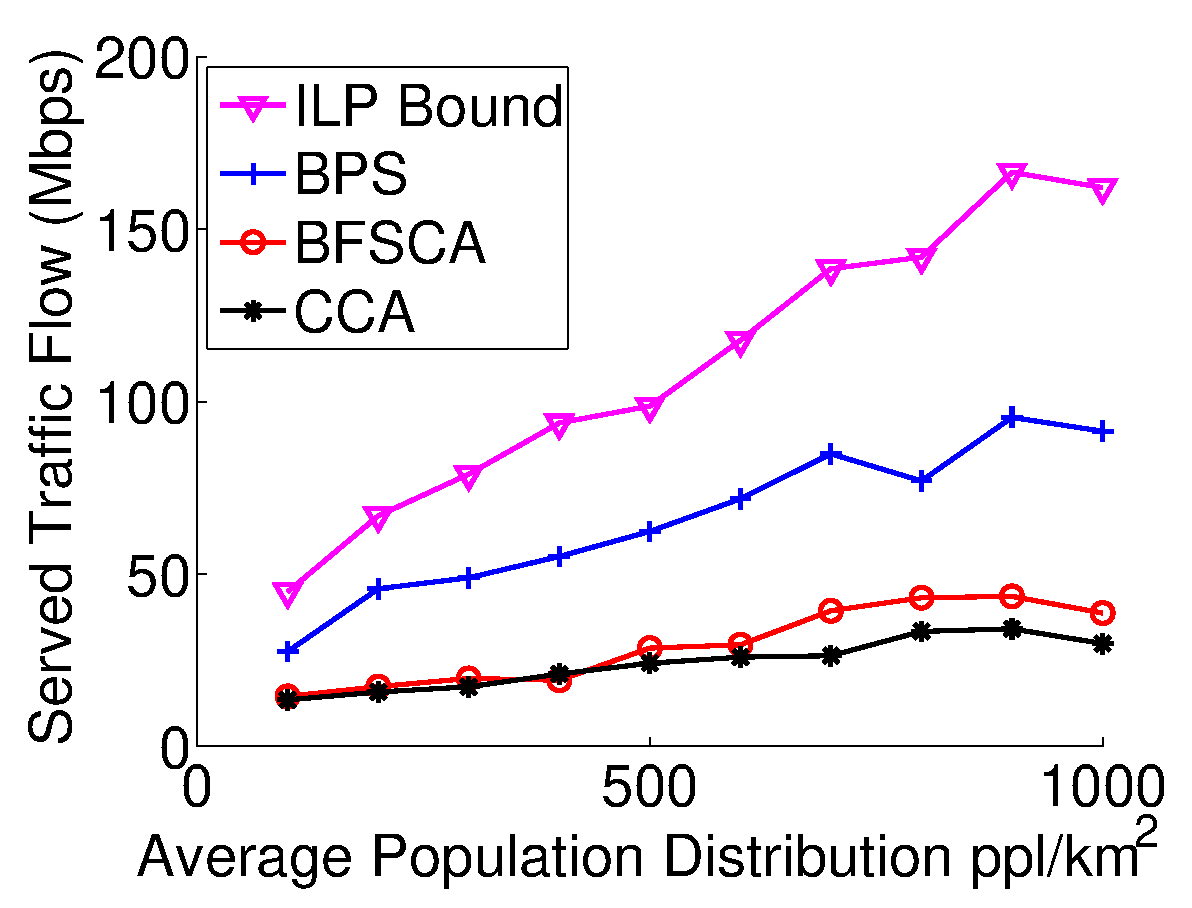
\includegraphics[width=74mm]{figures/maxtpt}
\vspace{-0.1in}
\caption{Max Tpt under Demand Bound}                                                                               
\label{fig:maxtpt}
%\vspace{-0.0in}
\end{figure}

To evaluate the performance in different size of network, we assign the demand of each node $5MB/s$ as demand upper bound, and vary the number of nodes in the regular grid network. The performance of the algorithms are shown in ~\ref{fig:varysize}. 
\begin{figure}
%\vspace{-0.0in}
\centering
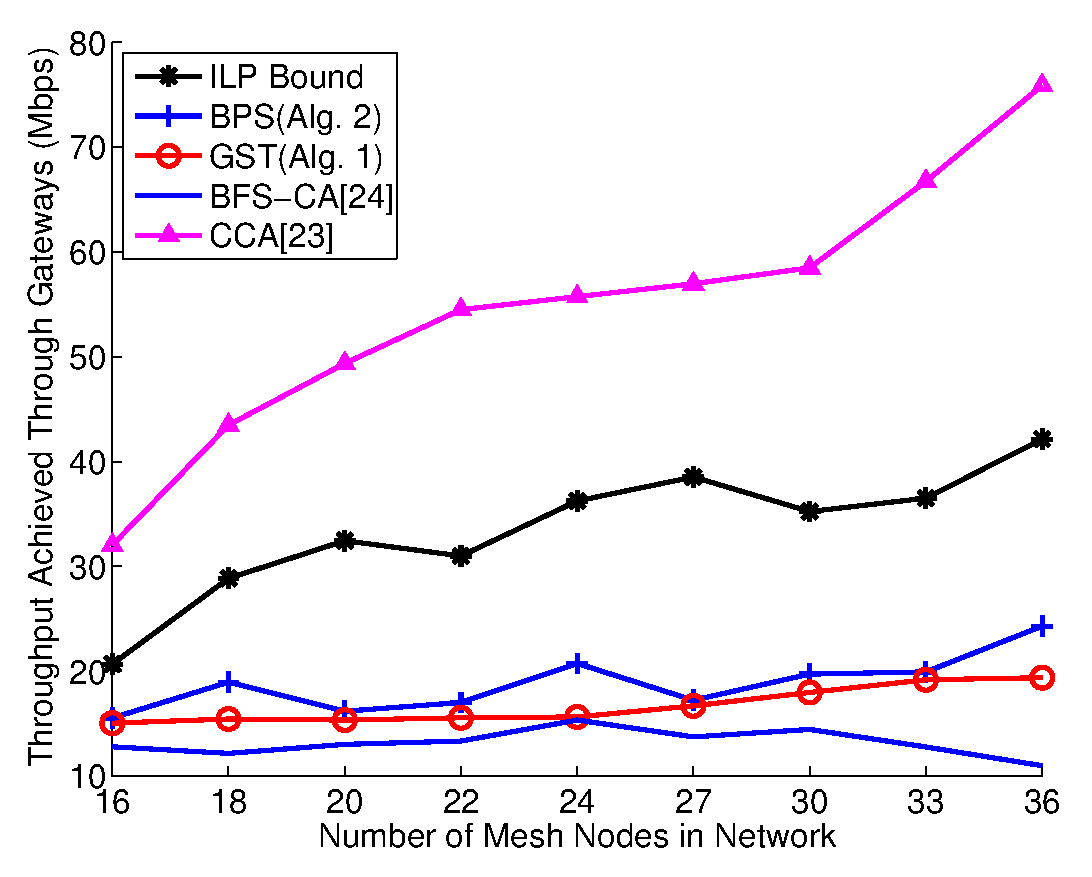
\includegraphics[width=74mm]{figures/varysize}
\vspace{-0.1in}
\caption{Max Tpt of Network Size}                                                                               
\label{fig:varysize}
%\vspace{-0.0in}
\end{figure}

\subsection{Min Conflict Weight}

~\emph{Conflict Weight} is the amount of links interfered by a single link ~\cite{JaPaPaQi03}. 










%\subsection{Performance Analysis of Algorithms}
\label{subsec:results}

We now investigate the performance of our proposed
multiband network placement algorithms in different scenarios.
First we analyze the performance of the two algorithms in a 7x7 regular grid whose mesh nodes could be installed on the cross points.
Then we put the algorithms on in-field network placment of TFA and Google network.




\section{Related Work}
\label{sec:related}
% Deployment problem 
There are significant challenges in wireless mesh network deployment,
such as user priorities, user behaviors, long term throughput estimation, 
interference and energy efficiency, etc.~\cite{tragos2013spectrum}
Previous works have recognize the impact of interference in wireless mesh network 
deployment is the key issue~\cite{tang2005interference,irwin2013resource,chieochan2013channel}.
To overcome the challenges, previous works have been done to optimize the 
deployment in increasing throughput, minimize resource, reducing interference,
etc~\cite{irwin2013resource,subramanian2008minimum,doraghinejad2014channel}.
Many works have studied the network deployment problem in multihop wireless networks
~\cite{jain2005impact,akyildiz2005wireless,raniwala2004centralized,tragos2013spectrum}.
Both static and dynamic network deployments have been discussed in previous works under
the 802.11 WiFi scenario~\cite{wu2006analysis,ramachandran2006interference,subramanian2008minimum}. 
However, all of the aforementioned works have not considered propagation variation of the 
diverse frequency bands among white space and WiFi, which we show are critical improving 
the performance of mesh networks. Frequency agility in multiband scenario brings more 
achieved channel capacity to wireless network deployment as well as more complexity of 
resolving the interference issues.

% White Space
To be used effectively, white space bands must ensure that available TV bands
exist but no interference exists between microphones and other devices~\cite{bahl2009white}. 
White space bands availability has to be known in prior of network deployment.
TV channels freed by FCC are fairly static in their channel assignment, 
databases have been used to account for white space channel availability 
(e.g., Microsoft's White Space Database~\cite{msdatabase}).
In fact, Google has even visualized the licensed white space channels 
in US cities with an API for research and commercial use~\cite{googledatabase}.
In contrast, we study the performance of mesh networks with a varying number 
of available white space channels at varying population densities, assuming 
such white space databases and mechanisms are in place. As FCC release these 
bands for research, many methods have been proposed to employ these frequency bands.
~\cite{bahl2009white} introduce WiFi like white space link implementation on USRP and 
link protocols. ~\cite{cui2013leveraging} discuss the point to point communication
in multiband scenario. In~\cite{filippini2013new}, white space band application is 
discussed in cognitive radio network for reducing maintenance cost. 
In this work, the objective is maximizing the served traffic flow of clients in the wireless network.






\section{Conclusion}
\label{sec:conclusion}
In this paper, we jointly considered the use of WiFi and white space bands application
for wireless networks deployments. 
Different from prior work, we first proposed a Multiband 
Access Point Estimation (MAPE) framework to estimate the number of access points required in 
a given region for wireless access network and Band-based Path Selection (BPS) algorithm for
backhual network based on in-field measurements for wireless access network. 
We then performed spectrum utilization measurements in the DFW metropolitan and surrounding areas 
to drive these framework and find the influence of white spaces on network costs in these representative areas. 
%
%Further, we investigate different 
%band combinations in two population densities to show that greater access to white space 
%channels have greater total savings of mesh nodes when the total number of channels used 
%in the network is fixed (i.e., given a total number of allowable WiFi and white space channels). 
Through extensive analysis across varying population density and channel combinations across bands, 
we show that white space bands can reduce the number of access points by 1650\%
and 660\% in rural and sparse urban areas versus the same cost savings are not achieved in dense urban 
and downtown type area. As the population and spectrum utilization increase, the cost savings of 
white space bands diminish to the point that WiFi-only channel combinations can be optimal.
The simulation shows that our BPS algorithm can achieve 180\% the served user demand versus previous 
multi-channel, multi-radio solutions in multiband scenarios, since we leverage diverse propagation 
characteristics offered by WiFi and white space bands. Moreover,we quantify the degree to which the joint 
use of these bands can improve the served user demand. Our BPS algorithm shows that WhiteMesh topologies 
can achieve up to 160\% of the served traffic flow of similar WiFi or white-space-only configurations.
% Future work
%In the future, we will consider the heterogeneous access points and traffic demand scenarios
%in wireless network deployments.





\bibliographystyle{IEEEtran}

\bibliography{whitemesh}

\end{document}
%This is never printed
